\subsubsection{Riparo autocostruito a tetto apribile \textit{a fiore}}
Questa realizzazione \`e sicuramente la pi\`u economica e necessita di:
\begin{itemize}
	\item[->] Un telaio in acciaio in modo da costruire un serramento che si apra dal centro, come visibile in Fig.~\ref{SERR:FIORE};
\begin{figure}
	\centering
	\begin{subfigure}[b]{0.4\textwidth}
		\centering
		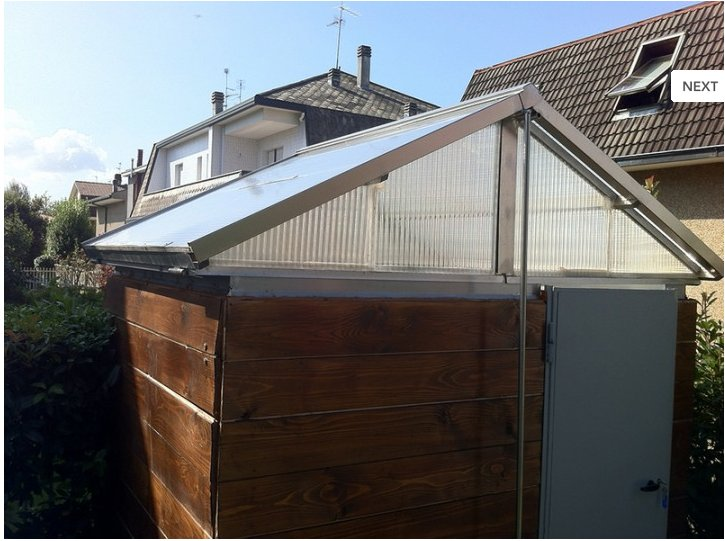
\includegraphics[width=120mm,angle=0,clip=,scale=0.5]{tetto1.jpeg}
		\caption{Struttura di esempio col tetto chiuso}
	\end{subfigure}
	\qquad\quad
	\begin{subfigure}[b]{0.4\textwidth}
		\centering
		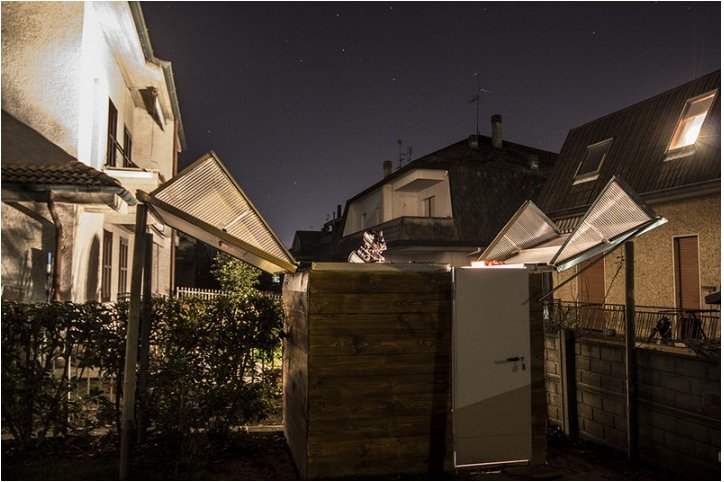
\includegraphics[width=120mm,angle=0,clip=,scale=0.5]{tetto2.jpeg}
		\caption{Struttura di esempio col tetto aperto e i supporti laterali}
	\end{subfigure}
	\caption{Modalit\`a di riparo con apertura a \textit{fiore}}
	\label{SERR:FIORE}
\end{figure}
	\item[->] In Fig.~\ref{SERR:FIORE} il telaio \`e stato riempito con del plexiglass. Nel nostro caso verr\`a saldata una lamiera coibentata.
	\item[->] La struttura del tetto sar\`a posizionata sopra ad un cubo $2m\times2m\times1.50m$
	      che rappresenter\`a la sede del telescopio. La sua realizzazione sar\`a sempre in lamiera coibentata supportata da quattro pilastrini che sorgerebbero ai vertici della base del quadrato.
      \item[->] Per evitare infiltrazioni d'acqua dal pavimento si \`e pensato di realizzare un pavimento in materiale composito, uno strato in legno, uno strato in gomma e nuovamente uno strato in legno. Questo sar\`a fissato con delle ganasce (in modo da non forare il tetto) alle piottole del tetto. Tutta la struttura, oltre ad essere fissata alla sua base, sar\`a fissata ulteriormente, sempre con delle ganasce che si stringono a vite, al corrimano del terrazzo che fa angolo (si veda la pianta Fig.~\ref{PIANTA}). \`E opportuno che il riparo venga dotato anche di una presa d'aria che permetta il flusso d'aria (evitando il ristagno d'aria quindi la formazione delle muffe).`
      \item[->] Al riparo dovr\`a arrivare \textbf{corrente elettrica} e un cavo di collegamento \textbf{ethernet}. La corrente sembra essere accessibile da pi\`u punti in particolar modo da un quadro elettrico gi\`a presente sul terrazzo (sotto ad una grande antenna), rimane da definire bene il persorso che fanno i cavi ethernet gi\`a presenti all'interno della struttura. Da un primo sopralluogo \`e sembrato che sia possibile accedere ad uno switch prossimo al terrazzo.

\end{itemize}
Una stima del prezzo del riparo si aggira intorno ai \textbf{5000euro}.

